Alle klasser i CSS-hovedenhedspakken er testet. De enkelte tests er beskrevet i det følgende afsnit.
Se det statiske klassediagram for at se sammenhængen mellem klasserne i figur \ref{fig:CSS_hovedenhed_Class_Static}.

% Timer
\subsubsection{Timer}
Timer klassen er testet med programmet ''Timer Test.cpp'' som ligger i kildekoden til klassen.
Programmet opretter et objekt af Timer typen og starter et endeløst loop som tænder timeren i 1 sekund og slukker den i 1 sekund.

\textbf{Opstilling}

En oscilloscope probe sættes på PD5 på et STK500 kit som har programmet kørende.


%På figur \ref{fig:Test_CSS_Timer_scope} vises et oscilloscope billede målt på udgangen af timeren PD5.

%\begin{figure}[!htb]
%	\centering
%     {\includegraphics[width=\textwidth]{billeder/SWTest/CSS_Timer_scope}}
%     \caption{Oscilloscope måling på udgangen af Timer1 på STK500 kit.}
%     \label{fig:Test_CSS_Timer_scope}
%\end{figure}

% UART
\subsubsection{UART}
UART klassen er testet med programmet ''UART Test.cpp'' som ligger i kildekoden til klassen.
Programmet starter med at sende en streng over RS232 interfacet. Her efter afventer den at modtage en hel kommando. Når denne er modtaget sendes den retur.

\textbf{Opstilling}

Testprogrammet ligges på et STK500 kit.
En computer forbindes med STK500 kittet over RS232 Spare porten (Sub-D).
En jumper forbinder headeren RXD med PD0 og TXD med PD1.
Start et terminalprogram op indstillet til 9600 buad, 8 databit, 1 stopbit og ingen paritet.
Reset STK500 og programmet starter.

Først modtages strengen ''CSS hovedenhed\textbackslash r\textbackslash n''.
Send igennem terminal her efter, én karakter af gangen: ''A0101\textbackslash r''. Dette modtages igen som svar.
Send igen, én karakter af gange: ''D0011\textbackslash r''. Dette modtages igen som svar.

% CircBuffer
\subsubsection{CircBuffer}
CircBuffer klassen er testet med programmet ''CircBuffer Test.cpp'' som ligger i kildekoden til klassen.

\textbf{Opstilling}

Test programmet ligges på et STK500-kit.
En computer forbindes med STK500-kittet over RS232 Spare porten (Sub-D).
En jumper forbinder headeren RXD med PD0 og TXD med PD1.
Start et terminalprogram op indstillet til 9600 buad, 8 databit, 1 stopbit og ingen paritet.
Reset STK500 og programmet starter.

Det sender først de to index fra klassen som peger på den næste plads og den plads som skal aflæses næste gang adskilt af mellemrum.
Denne forventes at være ''0 0''. Her efter indsættes en karakter ('A') og index tallene udskrives igen. Denne gang forventes det at NextIndex er steget, så ''1 0''. Karakteren læses så ud igen med get()-metoden og denne sendes efterfulgt af index tallene. Disse forventes nu at være ''1 1''.

Bufferen fyldes til sidste med 'B' 1.5 gange, altså overfyldes den. Den afsluttes med et 'C'. Her efter sendes alle værdier i bufferen retur indtil den rammer 'B'et. Der forventes at komme 52 'B'er ud og et 'C'. Dette viser at det er en cirkulær buffer da de ældste værdi er overskrevet.
Til sidst udskrives index tallene. Da de er castede fra ints til chars modtages ''6 6'' hvilket svare til 54.

% RS232IF
\subsubsection{RS232IF}
RS232IF klassen er testet med programmet ''RS232IF Test.cpp'' som ligger i kildekoden til klassen.

\textbf{Opstilling}

Test programmet ligges på et STK500 kit.
En computer forbindes med STK500 kittet over RS232 Spare porten (Sub-D).
En jumper forbinder headeren RXD med PD0 og TXD med PD1. Et 8-ledet fladkabel sættes mellem LEDS og PORTB på STK500-kittet.
Start et terminalprogram op indstillet til 9600 buad, 8 databit, 1 stopbit og ingen paritet.
Reset STK500 og programmet starter.

Først afsender programmet de tre kommandoer som kan sendes til computeren. Hhv. advisering om babyalarm og svar på loginstatus.
Forventet modtages ''SB9999\textbackslash r'', ''ST9999\textbackslash r'' og ''SF9999\textbackslash r''.
Her efter afventer programmet en fuld kommando. Hvis den stemmer overens med en af de mulige UC udskrives nummeret binært på LEDerne på STK500-kittet og den sender den modtagende adresse retur.
Testes med kommandoerne i tabel \ref{table:Test_RS232IF_kommandoer} og svar modtages. Bemærk at i Atmels terminal miljø skal karakterende sendes enkeltvis.

\begin{table}[h]
	\caption{Test kommandoer og svar for RS232IF modul test}
	\centering
	\begin{tabular}{|c|c|c|}
		\hline 
		\textbf{Kommando ASCII} & \textbf{Kommando HEX} & \textbf{Svar} \\ 
		\hline 
		SA1010\textbackslash r & 53 41 31 30 31 30 0D & 1010 LED1 lyser (UC2) \\ 
		\hline 
		sd0011\textbackslash r & 73 64 30 30 31 31 0D & 0011 LED1 og LED0 lyser (UC3) \\ 
		\hline 
		sL9999\textbackslash r & 73 4C 39 39 39 39 0D & LED0 lyser (UC1) \\ 
		\hline 
	\end{tabular} 
	\label{table:Test_RS232IF_kommandoer}
\end{table}

% X10IF
\subsubsection{X10IF}
X10IF klassen er testet med programmet ''X10IF Test.cpp'' som ligger i kildekoden til klassen.

\textbf{Opstilling}

Test programmet ligges på et STK500 kit.
En PC forbindes med STK500-kittet over RS232 Spare porten (Sub-D).
En jumper forbinder headeren RXD med PD0 og TXD med PD1. Et 8-ledet fladkabel sættes mellem LEDS og PORTB på STK500 kittet. Jumper forbinder SW0 med PD2.
Start et terminalprogram op indstillet til 9600 buad, 8 databit, 1 stopbit og ingen paritet.
Reset STK500 og programmet starter.

Først sendes antallet af kommandoer i kø som ASCII tal. Der efter indsættes kommandoen aktiver i køen og antallet sendes igen. Dette gentages for deaktiver kommandoen. Der forventes udskrevet ''0 1 2''.
Her efter tømmes bufferen og alle værdier sendes. Disse er formateret i X10 formatet og kontrolleres i henhold til protokol beskrivelsen.
Interrupt delen testes når LED7 lyser. Her er det muligt, ved tryk på SW0 at få alle dioderne til at lyse i 0,25 sekunder.
 
% ZeroCrossInt
\subsubsection{ZeroCrossInt}
ZeroCrossInt ISR er testet med programmet ''ZeroCrossInt Test.cpp'' som ligger i kildekoden til funktionen.

\textbf{Opstilling}

Test programmet ligges på et STK500 kit.
Jumper forbinder PD2 og PB0. Et oscilliscope forbindes med to prober til PB2 og PD5.
Reset STK500 og programmet starter.

Først lægges to kommandoer i kø, hhv. aktiver og deaktiver. Her efter genereres et firkantsignal på 250 Hz som føres ind på INT0 benet for at starte ISR funktionen.

Med scopet kan så måles de rette bursts ud fra kommandoerne. På figur \ref{fig:Test_CSS_ZeroCross_sender1} kan man se de to kommandoer afsendt. Det gule signal er 120 kHz bursts svarende til X10 formaterede bits. Det grønne signal er det simulerede ZeroCross signal. I den øverste del kan man se aktiver kommandoen sendt to gange og i den nederste del er der zoomet ind på den sidste del. Dette stemmer overnes med protokol beskrivelsen.

På figur \ref{fig:Test_CSS_ZeroCross_sender2} kan man se både aktiver og deaktiver kommandoen.
Bursts signalet skal være på 120 kHz. 

Figur \ref{fig:Test_CSS_ZeroCross_Bursts} kan man se bursts signalet. Bemærk at frekvensen er lidt højerer end forventet (134 kHz). Dette skyldes at den interne timer i STK500-kittet ikke kan komme 120 kHz nærmere.
Reaktionstiden for programmet er målt i figur \ref{fig:Test_CSS_ZeroCross_Delay}. Her kan det konstateres at fra der kommer et toggle på INT0 indgangen går der 32 us før burstet sendes afsted.

\begin{figure}[!htb]
	\centering
     {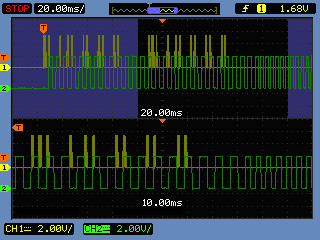
\includegraphics[width=0.8\textwidth]{billeder/SWTest/X10IF_Test_Afsend_1_kommando}}
     \caption{X10 Aktiver kommando. Oscilloscope måling, PB2 (Grøn) og PD5 (Gul)}
     \label{fig:Test_CSS_ZeroCross_sender1}
\end{figure}

\begin{figure}[!htb]
	\centering
     {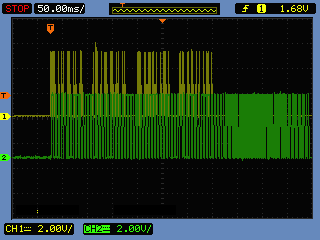
\includegraphics[width=0.8\textwidth]{billeder/SWTest/X10IF_Test_Afsend_2_kommandoer}}
     \caption{X10 Aktiver og deaktiver kommandoer. Oscilloscope måling, PB2 (Grøn) og PD5 (Gul)}
     \label{fig:Test_CSS_ZeroCross_sender2}
\end{figure}

\begin{figure}[!htb]
	\centering
     {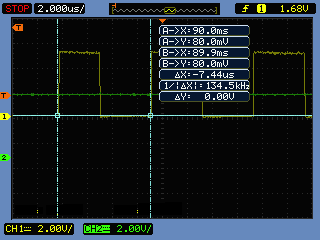
\includegraphics[width=0.8\textwidth]{billeder/SWTest/X10IF_Test_Burst}}
     \caption{120 kHz bursts. Oscilloscope måling, PB2 (Grøn) og PD5 (Gul)}
     \label{fig:Test_CSS_ZeroCross_Bursts}
\end{figure}

\begin{figure}[!htb]
	\centering
     {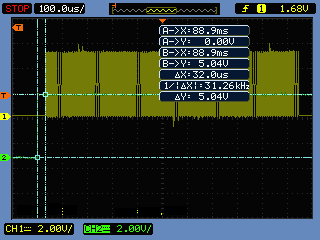
\includegraphics[width=0.8\textwidth]{billeder/SWTest/X10IF_Test_Delay}}
     \caption{Reaktionstid. Oscilloscope måling, PB2 (Grøn) og PD5 (Gul)}
     \label{fig:Test_CSS_ZeroCross_Delay}
\end{figure}